\section{Machine learning}
\begin{frame}{Late 2000s - machine learning dominates}
	\begin{columns}
		\begin{column}{.5\textwidth}
			\begin{figure}
				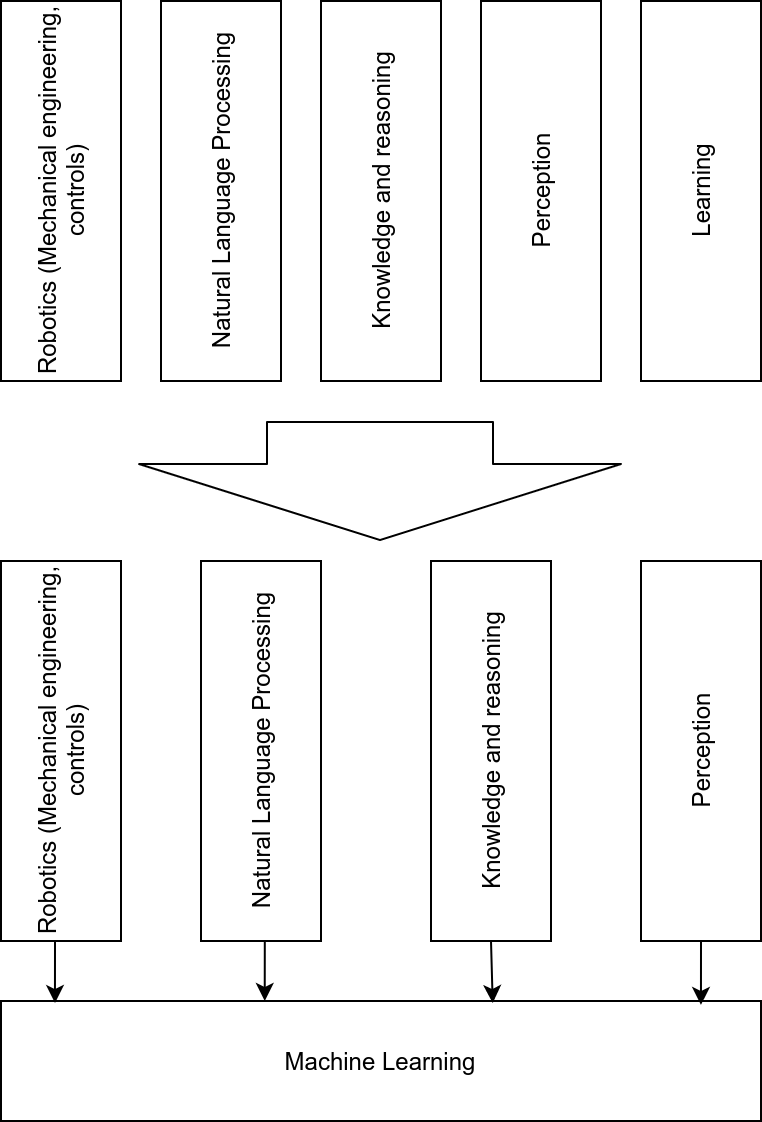
\includegraphics[width=.75\textwidth, center]{figures/agent_components_2}
			\end{figure}
		\end{column}
		\begin{column}{.5\textwidth}
			{\small 
				\begin{itemize}
					\item Image classification, localization and segmentation 
					\item Neural machine translation, question answering, summary. 
					\item Game playing, helicopter flying (stunts)
					\item Planning, self driving cars 
					\item Text, audio and video processing, generation 
					\item $\dots $
				\end{itemize}
			}
		\end{column}
	\end{columns}
\end{frame}
\begin{frame}{Machine learning models}
	\begin{columns}
		\begin{column}{.5\textwidth}
			\begin{block}{Models}
				\begin{itemize}
					\item Build a model of the world  
					\item Infer/predict using the model. 
				\end{itemize}
			\end{block}
		\end{column}
		
		\begin{column}{.5\textwidth}
			\begin{block}{Machine learning}			
				\begin{itemize}
					\item Supervised learning 
					\item Unsupervised learning 
					\item Reinforcement learning 
				\end{itemize}
			\end{block}
		\end{column}
	\end{columns}
\end{frame}

\begin{frame}{Supervised learning}
	\begin{columns}
		\begin{column}{.5\textwidth}
			\begin{figure}
				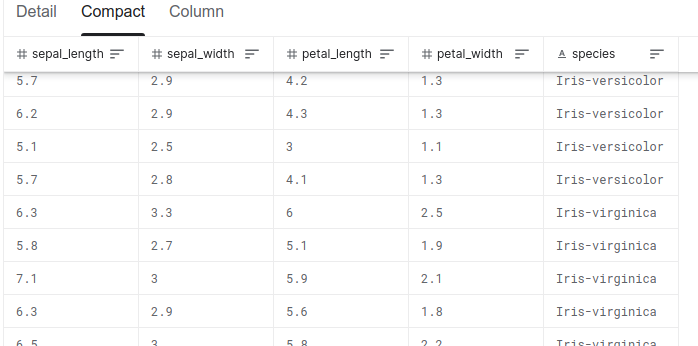
\includegraphics[width=1\textwidth, center]{figures/iris_dataset_1}
				
			\end{figure}
		\end{column}
		\begin{column}{.5\textwidth}
			\begin{figure}
				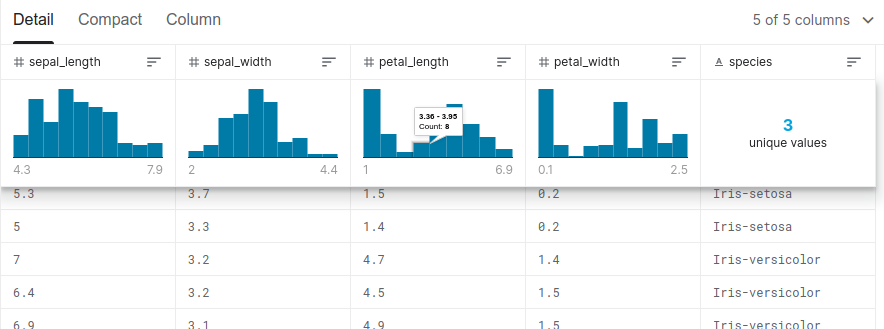
\includegraphics[width=1\textwidth, center]{figures/iris_dataset_2}
			
			\end{figure}
		\end{column}
	\end{columns}
	\begin{center}
		{\tiny Source:{\em https://www.kaggle.com/arshid/iris-flower-dataset?select=IRIS.csv}}
	\end{center}
\end{frame}

\begin{frame}{Supervised learning process flow}
	\begin{columns}
		\begin{column}{.5\textwidth}
			\begin{figure}
				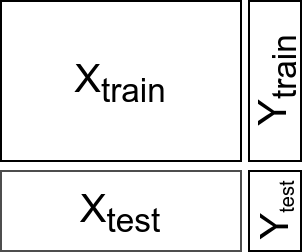
\includegraphics[width=.85\textwidth, center]{figures/ml_1_data}
				\caption*{Data}
			\end{figure}
		\end{column}
		\begin{column}{.5\textwidth}
			\begin{figure}
				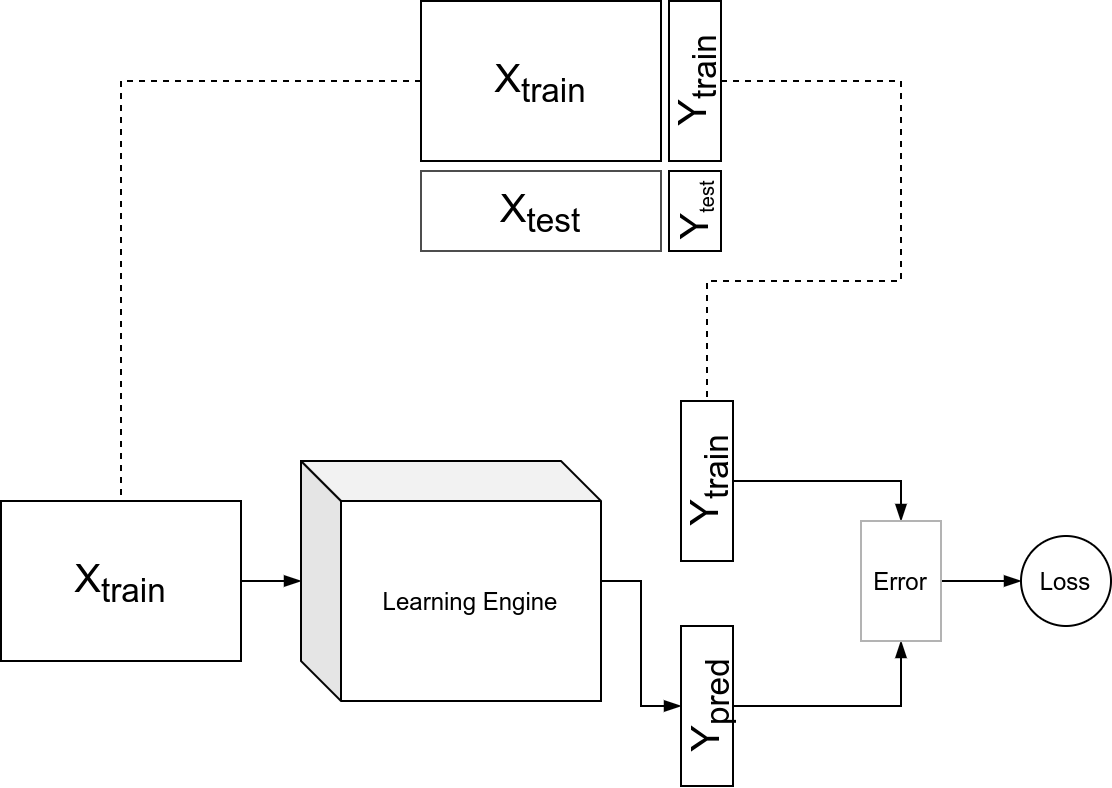
\includegraphics[width=1.\textwidth, center]{figures/ml_1_train}
				\caption*{Training}
			\end{figure}
		\end{column}
	\end{columns}
\end{frame}

\begin{frame}{Supervised learning process flow}
	\begin{columns}
		\begin{column}{.5\textwidth}
			\begin{figure}
				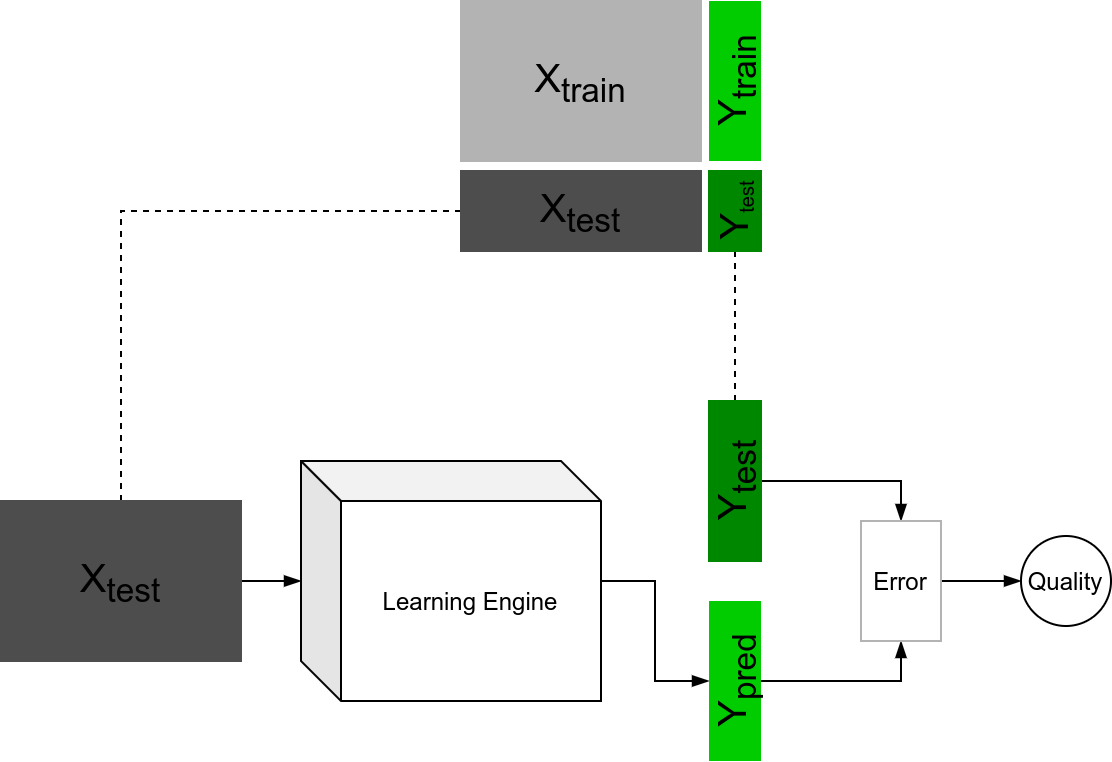
\includegraphics[width=1.\textwidth, center]{figures/ml_1_test}
				\caption*{}
			\end{figure}
		\end{column}
		\begin{column}{.5\textwidth}
			\begin{figure}
				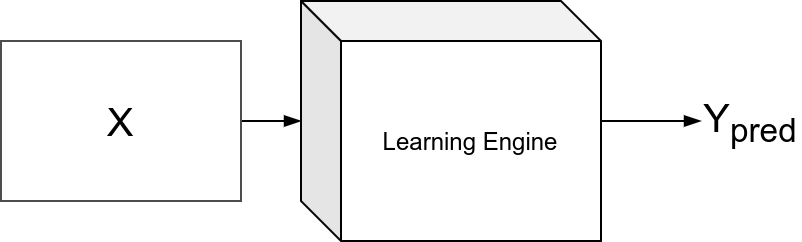
\includegraphics[width=1.\textwidth, center]{figures/ml_1_infer}
				\caption*{}
			\end{figure}
		\end{column}
	\end{columns}
	\begin{columns}
		\begin{column}{.5\textwidth}
			\begin{center}
				Testing
			\end{center}
		\end{column}
		\begin{column}{.5\textwidth}
			\begin{center}
				Predicting
			\end{center}
		\end{column}
	\end{columns}
\end{frame}


\begin{frame}{Machine learning}
	\begin{columns}
		\begin{column}{.5\textwidth}
			\begin{block}{Unsupervised learning}
				\begin{itemize}
					\item Training a model to find patterns in a dataset, typically an unlabeled dataset.
					\item Learning how to extract {\em interesting} features.
					\item Learning data distribution for generating data.
				\end{itemize}
			\end{block}
		\end{column}
		\begin{column}{.5\textwidth}
			\begin{block}{Reinforcement learning}
				A family of algorithms that learn an optimal policy, whose goal is to maximize return when interacting with an environment. 
				\begin{figure}
					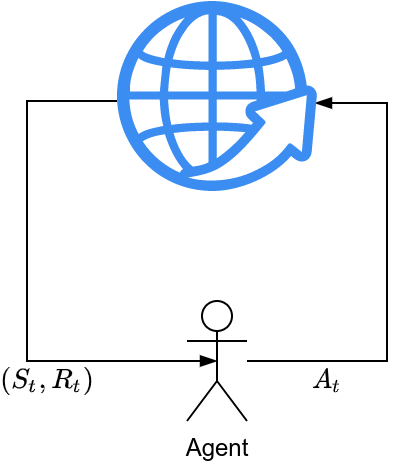
\includegraphics[width=.4\textwidth, center]{figures/RL_1}
				\end{figure}
			\end{block}
		\end{column}
	\end{columns}
\end{frame}